\documentclass[11pt,UTF8]{report}

\usepackage{ctex}

\usepackage{listings}
\usepackage{xcolor}

\usepackage{graphicx}
\usepackage{amsmath}

\usepackage[colorlinks, linkcolor=red, anchorcolor=blue, citecolor=green]{hyperref}

\definecolor{codegreen}{rgb}{0,0.6,0}
\definecolor{codegray}{rgb}{0.5,0.5,0.5}
\definecolor{codepurple}{HTML}{C42043}
\definecolor{backcolour}{HTML}{F2F2F2}
\lstdefinestyle{sql1}{% sql1 是格式的名字
	language=SQL,
	backgroundcolor=\color{backcolour},   
	commentstyle=\color{codegreen},
	keywordstyle=\color{codepurple},
	numberstyle=\footnotesize\color{black},
	stringstyle=\color{codepurple},
	basicstyle=\footnotesize,
	breakatwhitespace=false, 
	breaklines=true,                 
	captionpos=b,                    
	keepspaces=true,                 
	numbers=left, 
	showspaces=false,                
	showstringspaces=false,
	showtabs=false,
	tabsize=2      
}

\renewcommand\thesection{\arabic{section}}

\title{数据库系统概论项目报告}
\author{孙昭言 2018011308}
\begin{document}
	\maketitle
	
	\section{系统概述}
	该单用户数据库管理系统是我独自实现的,项目的Github地址为:\url{https://github.com/Curtis001/Single-user-DBMS}
	\subsection{必做功能}
	\begin{itemize}
		\item 记录管理模块
		\item 索引模块,支持联合索引的创建和删除
		\item 系统管理模块,支持INT, CHAR, DATE, DECIMAL等数据类型,支持主外键的创建和删除()包括完整性约束),支持列的添加、修改和删除
		\item 查询解析模块,支持增删查改等基本操作,对系统鲁棒性和错误报告做了较多处理
	\end{itemize}
	
	\subsection{选做功能}
	\begin{itemize}
		\item CHECK, UNIQUE INDEX等属性完整性约束
		\item 多表连接
		\item 聚合函数COUNT, AVG, SUM, MIN, MAX
		\item LIKE模糊匹配
		\item IN范围匹配,支持数组或SELECT子句结果
		\item 对WHERE子句结合索引进行查询优化
		\item +, -, *, /, AND, OR等运算符组成复杂表达式
	\end{itemize}
	
	\section{系统架构设计}
	\begin{figure}[!ht]
		\centering
		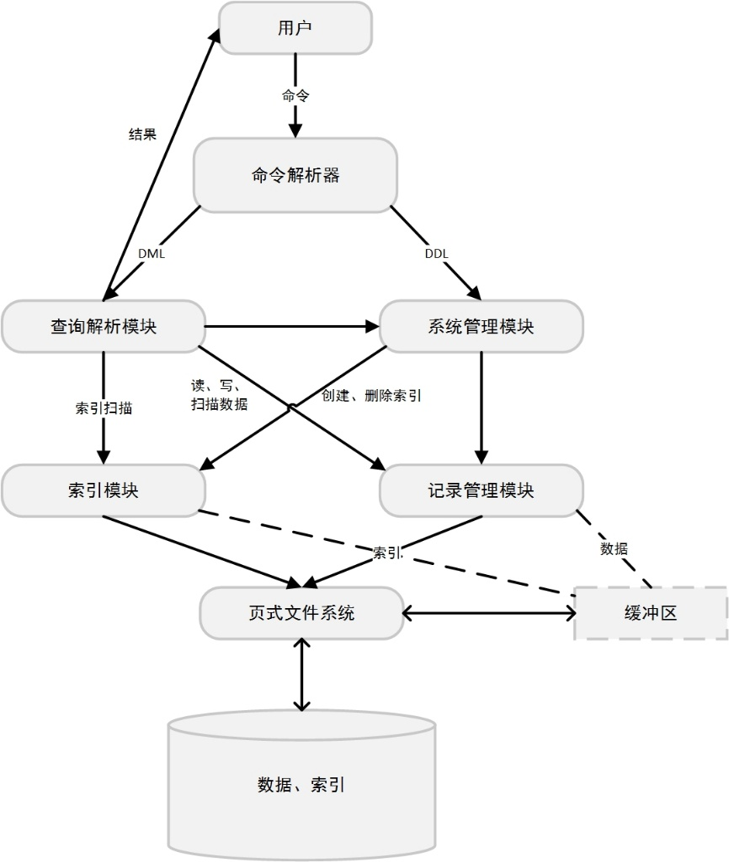
\includegraphics[width=0.9\textwidth]{structure}
		\caption{系统架构设计图}
		\label{fig:structure}
	\end{figure}
	
	系统架构与《 数据库大作业详细说明》 完全一致。
	
	\section{主要模块设计原理}
	
	\subsection{记录管理模块}
	表的第0列是隐含的具有唯一性的rid,其后是表的模式中的各列。表的每一行中各列的值紧密排列,每一列的值的第一个字节表示该值是否为null。当某一行的值有效时,其第0列为该行的rid;否则,其第0列为下一个空闲行的地址。表头中记录了第一个空闲行的地址。这样所有的空闲行组成一个链表,而且可以根据第0列的rid和该行的地址是否对应判断该行的值是否有效。删除某一行时,将该行的位置添加到链表表头,从而提高缓存的命中率。
	
	\subsection{索引管理模块}
	该模块使用了开源的B+树模块。B+树的每一个结点存储了压缩后的key值和rid值。在打开表时,索引被载入,而且根据表的模式解释压缩后的key值来比较大小;关闭表时,索引被写回。其中,null值认为最小,而且引入人为规定的最大值辅助筛选;所有key值相同时比较rid的大小。该模块不仅支持多列索引,而且可以只利用多列索引的前若干列进行筛选。
	
	\subsection{系统管理模块}
	每个数据库对应data文件夹下的一个文件夹,每个表又对应其下的一个文件夹,其中包括表的内容对应的文件tb和各索引对应的文件。主键、外键、唯一索引等特殊索引分别存储在表的文件夹下的相应文件夹中。表的模式存储在tb的第一页中,表项的默认值存储在表的第二页第一行,表的索引信息通过扫描其对应目录的文件情况恢复/存储。
	
	修改表的模式时,表头会被修改,之后根据新的表头重建tb文件和所有的索引文件。
	
	\subsection{SQL解析器}
	sqlparser使用flex和bison工具实现, 其语法大致与《 parser文法规则 》相同,但还增加了对选做功能的支持。 
	
	\subsection{查询处理模块}
	INSERT和UPDATE执行前会检查记录是否满足check、not null、唯一性索引、外键等约束,也会检查相应列是否符合数据类型要求。
	
	运算符组织成树形结构,叶节点可以是常数或表的某列,称为运算树。实际计算时,通过给定各表的rid值从而确定表的某列的值,进而自下而上计算出结果。运算符支持逻辑运算的短路运算,支持运算数进行兼容的类型转换,支持将整棵树转换为字符串的形式进行存储/恢复。
	
	WHERE子句对于多表的筛选结果会被表示成rid序列的集合,对应每个表中的某一行组合在一起。WHERE子句会先按照OR进行划分;对于每个AND子句,多个表会逐个计入考虑;每添加一个表时,遍历现有rid序列的集合,对每个rid序列遍历新表的rid,并将它们组合后的结果合并成为新的rid序列集合。在遍历新表的rid时,我通过限制计算在运算树上的传播,实质上使用那些只涉及现有表的条件进行筛选。
	
	我还尽可能使用索引对查询进行优化。对于建立在(col1, col2, col3)上的多列索引,如col1=val1 AND col2 op val2形式的条件也可以使用索引进行筛选。对于 col1 op col2 形式的条件,如果col2对应的表t2出现在col1对应的表t1之前,则在遍历t1时可以认为col2值为常数,从而也可以使用col1上的索引。
	
	
	\section{实验结果}
	本项目需要依赖flex/bison工具,并且需要编译器支持C++11特性,使用cmake 可以进行自动构建。
	
	本项目在验收时通过了必做功能和绝大多数的选做功能测例。部分选做功能展示如下:
	\begin{lstlisting}[style=sql1]
		create table REGION_2 (R_REGIONKEY INT NOT NULL, R_NAME CHAR(25) NOT NULL, R_COMMENT VARCHAR(152), PRIMARY KEY(R_REGIONKEY), CHECK(R_REGIONKEY in (1, 3, 5, 6, 9) OR R_NAME > R_COMMENT));\end{lstlisting}
	\begin{lstlisting}[style=sql1]
		update lineitem_2 set L_TAX = (L_QUANTITY + L_EXTENDEDPRICE * L_DISCOUNT) * 3.0 where L_ORDERKEY < 5;\end{lstlisting}
	上述测例分别检验了CHECK约束和复杂表达式的实现,sql文件夹中有更多的针对选做功能的测例。
	
	\section{参考文献}
	\begin{itemize}
		\item 《数据库大作业详细说明》
		\item SimpleDB by Harry Chen \url{https://github.com/Harry-Chen/SimpleDB}
		\item TrivalDB by 周聿浩 \url{https://github.com/miskcoo/TrivialDB}
		\item MyDB by Zhengxiao Du and Yifan Wu \url{https://github.com/duzx16/MyDB}
		\item STX B+ Tree Template \url{https://panthema.net/2007/stx-btree}
	\end{itemize}
\end{document}
